%%%%%%%%%%%%%%%%%%%%%%%%%%%%%%%%%%%%%%%%%
% Beamer Presentation
% LaTeX Template
% Version 1.0 (10/11/12)
%
% This template has been downloaded from:
% http://www.LaTeXTemplates.com
%
% License:
% CC BY-NC-SA 3.0 (http://creativecommons.org/licenses/by-nc-sa/3.0/)
%
%%%%%%%%%%%%%%%%%%%%%%%%%%%%%%%%%%%%%%%%%

%----------------------------------------------------------------------------------------
%	PACKAGES AND THEMES
%----------------------------------------------------------------------------------------

\documentclass{beamer}

\mode<presentation> {

% The Beamer class comes with a number of default slide themes
% which change the colors and layouts of slides. Below this is a list
% of all the themes, uncomment each in turn to see what they look like.

%\usetheme{default}
%\usetheme{AnnArbor}
%\usetheme{Antibes}
%\usetheme{Bergen}
%\usetheme{Berkeley}
%\usetheme{Berlin}
%\usetheme{Boadilla}
%\usetheme{CambridgeUS}
%\usetheme{Copenhagen}
%\usetheme{Darmstadt}
%\usetheme{Dresden}
%\usetheme{Frankfurt}
%\usetheme{Goettingen}
%\usetheme{Hannover}
%\usetheme{Ilmenau}
%\usetheme{JuanLesPins}
%\usetheme{Luebeck}
%\usetheme{Madrid}
%\usetheme{Malmoe}
%\usetheme{Marburg}
%\usetheme{Montpellier}
%\usetheme{PaloAlto}
%\usetheme{Pittsburgh}
%\usetheme{Rochester}
%\usetheme{Singapore}
%\usetheme{Szeged}
\usetheme{Warsaw}

% As well as themes, the Beamer class has a number of color themes
% for any slide theme. Uncomment each of these in turn to see how it
% changes the colors of your current slide theme.

%\usecolortheme{albatross}
%\usecolortheme{beaver}
%\usecolortheme{beetle}
%\usecolortheme{crane}
%\usecolortheme{dolphin}
%\usecolortheme{dove}
%\usecolortheme{fly}
%\usecolortheme{lily}
%\usecolortheme{orchid}
\usecolortheme{rose}
%\usecolortheme{seagull}
%\usecolortheme{seahorse}
%\usecolortheme{whale}
%\usecolortheme{wolverine}

%\setbeamertemplate{footline} % To remove the footer line in all slides uncomment this line
%\setbeamertemplate{footline}[page number] % To replace the footer line in all slides with a simple slide count uncomment this line

\setbeamertemplate{navigation symbols}{} % To remove the navigation symbols from the bottom of all slides uncomment this line
}

\usepackage{graphicx} % Allows including images
\usepackage{booktabs} % Allows the use of \toprule, \midrule and \bottomrule in tables
\usepackage{listings}
\usepackage[font=scriptsize,labelfont=bf]{caption}
\usepackage{caption}
\usepackage{subcaption}
\usepackage{float}


\newenvironment{changemargin}[2]{% 
  \begin{list}{}{% 
    \setlength{\topsep}{0pt}% 
    \setlength{\leftmargin}{#1}% 
    \setlength{\rightmargin}{#2}% 
    \setlength{\listparindent}{\parindent}% 
    \setlength{\itemindent}{\parindent}% 
    \setlength{\parsep}{\parskip}% 
  }% 
  \item[]}{\end{list}} 

%----------------------------------------------------------------------------------------
%	TITLE PAGE
%----------------------------------------------------------------------------------------

\title[Testing and Refactoring NDT-MCL]{Testing and Refactoring NDT-MCL} % The short title appears at the bottom of every slide, the full title is only on the title page

\author{Aleksandar Mitrevski, Santosh Thoduka} % Your name
\institute[BRSU] % Your institution as it will appear on the bottom of every slide, may be shorthand to save space
{
Hochschule Bonn Rhein Sieg \\ % Your institution for the title page
\medskip
\textit{aleksandar.mitrevski@smail.inf.h-brs.de\\santosh.thoduka@smail.inf.h-brs.de} 
}
\date{June 24, 2014} % Date, can be changed to a custom date

\begin{document}

%----------------------------------------------------------------------------------------
%	PRESENTATION SLIDES
%----------------------------------------------------------------------------------------

\begin{frame}
\titlepage % Print the title page as the first slide
\end{frame}


\begin{frame}
\frametitle{Normal Distribution Transform - Monte Carlo Localisation}
\begin{itemize}
\item Normal distribution transform Monte Carlo localisation (NDT-MCL) [1] is a localisation algorithm whose goal is providing an estimate of the true position of a robot in a given environment
\item NDT-MCL parametrizes grid cells by Gaussian distributions, employing a so-called NDT representation as suggested by [2]
\item Localisation involves calculating a pose likelihood, updating particle weights, and resampling particles. 
\item The only difference in NDT-MCL is the likelihood calculation, such that $L2$-likelihood is used to express the discrepancy between the estimated and the actual robot pose.
\end{itemize}

\end{frame}

\begin{frame}
\frametitle{Node Description}
\begin{changemargin}{-1cm}{-1cm}
	\begin{figure}
    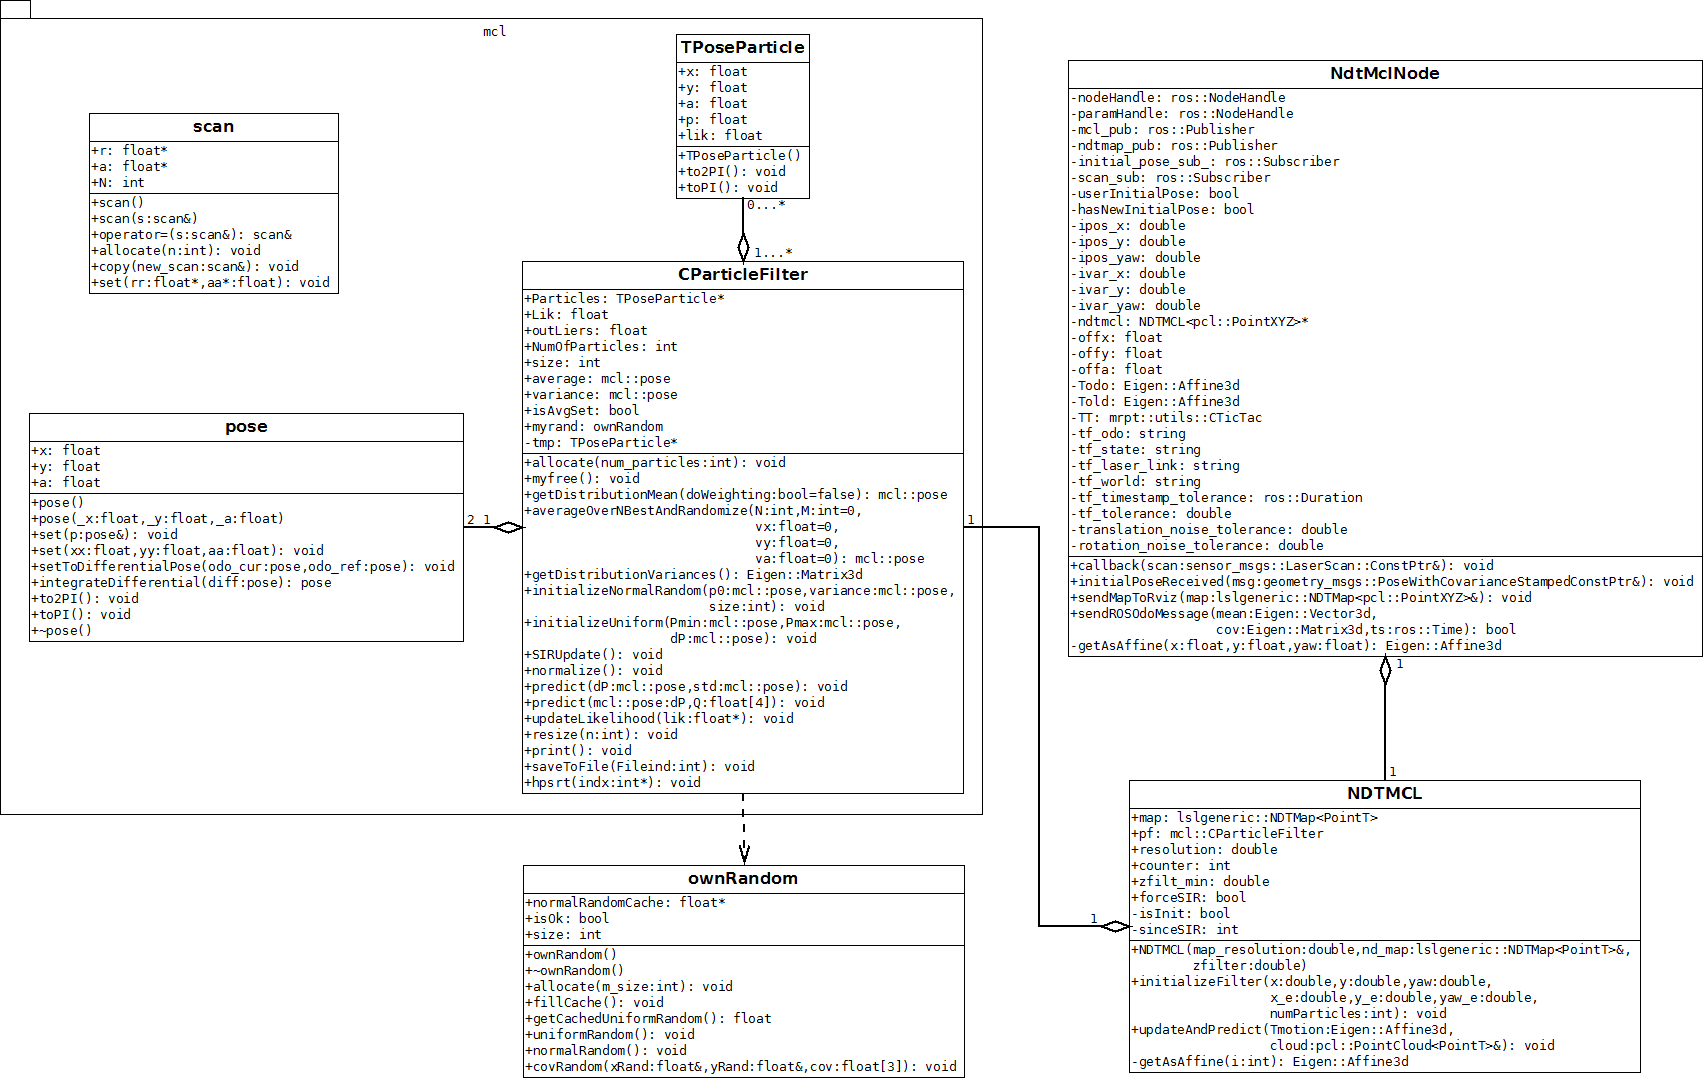
\includegraphics[height=0.74\textwidth]{ndtmcl.png}    
    \end{figure}
\end{changemargin}
\end{frame}

\begin{frame}
\frametitle{Implemented Modifications}
\begin{itemize}
\item Re-factored node as a class
\item Removed use of ground truth
\item Pose estimate published as transform between map and odom frame
\item Added parameters to the launch file - such as tf frames, translational and rotational tolerances, etc.
\end{itemize}
\end{frame}

\begin{frame}
\frametitle{Remaining Issues}
Tested localisation both in simulation and in a real environment
\begin{itemize}
\item Poor localisation during mapping using the NDT Fuser node (for mapping)
\item Map is not very accurate
\item Incorrect pose estimation while robot is stationary
\item Pose estimate ``jumps''
\end{itemize}
\end{frame}

\begin{frame}
\frametitle{Improvements and Future Work}
\begin{itemize}
\item More parameters should be exposed in the launch file so the node can be tuned to different platforms and environments if necessary
\item Resolution of map should be stored in the map file
\item Investigate compatibility with navigation planners
\item Port visualization to Rviz
\end{itemize}
\end{frame}

\begin{frame}
\frametitle{References}

	[1] J. Saarinen, H. Andreasson, T. Stoyanov, and A. J. Lilienthal, "Normal Distributions Transform Monte-Carlo Localization (NDT-MCL)," in {\it Intelligent Robots and Systems (IROS), 2013 IEEE/RSJ International Conference on}, Tokyo, Japan, 2013, pp. 382-389.\\

	[2] P. Biber, "The Normal Distributions Transform: A New Approach to Laser Scan Matching," in {\it Intelligent Robots and Systems, 2003. (IROS 2003). Proceedings. 2003 IEEE/RSJ International Conference on}, Las Vegas, NV, 2003, pp. 2743-2748.
\end{frame}

\end{document} 
